\graphicspath{{chapters/12/images/}}
\chapter{The isobaric ensembles}

\section{Introduction}
Why do we need to study the isobaric ensembles? 
The reason is that in MD we investigate systems of biological relevance, therefor all simulation should be run on constant temperature and pressure (atmospheric pressure).
  
	\subsection{Legendre transform of E}
	In order to get to that point, we first start by performing a Legendre transform of the energy (obtaining in this way the isobaric-isoentalpic ensemble). 
	The same reasoning was made when the canonical ensemble was introduced from microcanonical one. 
	The legendre transform will be taken of the energy, wrt to its derivative wrt to its entropy. 
	%We wanted to express the legendre tran of the energy in terms of the temperature, something that was exactly its derivate wrt to its entropy.
%We are introducing pressure, derv of the enrgy wrt to volume (-). We want to study this new energy, this will the the function of the number of molecules. Vol will be expressed in terms of the pressure.

	$$\tilde{f}(s) = f(x(s))-sx(s)\qquad s = f'(x)$$

	$$\tilde{E}(N, \frac{\partial E}{\partial V}, S) = E(N, V(P), S) - \biggl(\frac{\partial E}{\partial V}\biggr)_{N, S}V(N, \frac{\partial E}{\partial V}, S)$$
	

	We can define the \textbf{enthalpy}:

	$$H(N, P, S) = E(N, P, S) + PV(N, P, S)$$
	
	The quantity $H$ is called enthalpy. As it is usually done for thermodynamic potentials, we derive the expression for its differential form, that is equal to:
	
	$$dH = dE + PdV + VdP = TdS - PdV + \mu dN + PdV + VdP$$
	
	We know from the first principal of thermodynamics that $dE$ is equal to $TdS - PdV + \mu dN$, where $\mu$ is the chemical potential. Then we are left with the following expression: 

	$$dH = TdS + \mu dN + VdP$$

From this we can derive the usually derivatives:

	$$T = \biggl(\frac{\partial H}{\partial S}\biggr)_{N, P} \qquad \langle V\rangle = \biggl(\frac{\partial H}{\partial P}\biggr)_{N, S} \qquad \mu = \biggl(\frac{\partial H}{\partial N}\biggr)_{P, S}$$
	
	The volume is averaged because in this ensemble it is not fixed, but will vary. 

	\subsection{Legendre transform of A}
	 In the exact same way we can also apply the Legendre transform to the Helmholtz free energy, with the formulas being very similar to before: 

	$$\tilde{f}(s) = f(x(s))-sx(s)\qquad s = f'(x)$$
	
	Again it is a Legendre transform wrt its derivative wrt volume, so the derivative of A wrt to volume. We know that derivative is related to the pressure, being actually (-) pressure, so the LT will be equal to the Helmholtz itself, minus the derivative of $A$ wrt volume times volume, which will be expressed in terms of the derivative of $A$ wrt to volume:

	$$\tilde{A}(N, \frac{\partial A}{\partial V}, T) = A(N, V(P), T)- \biggl(\frac{\partial A}{\partial V}\biggr)_{N, T}V(N, \frac{\partial A}{\partial V}, T)$$
	
	A thermodynamic potential is derived, that is called \textbf{Gibbs free energy}:

	$$G(N, P, T) = A(N, P, T) + PV(N, P, T)$$

	The Gibbs free energy is the Legendre transform of the $A$, like the enthalpy is the Legendre transform of the energy. 
	Let's now take the infinitesimal variation of $G$: 
	$$dG = dA + PdV + VdP = -PdV + \mu dN - SdT + PdV + VdP$$
	
	Like before, the $PdV$ cancel out and we are left with the following expression:

	$$dG = \mu dN + VdP - SdT$$
	
	We can now tale the thermodynamic derivatives:

	$$S = -\biggl(\frac{\partial G}{\partial T}\biggr)_{N, P}\qquad\langle V\rangle = \biggl(\frac{\partial G}{\partial P}\biggr)_{N, T}\qquad \mu = \biggl(\frac{\partial G}{\partial N}\biggr)_{P, T}$$
	
	We obtained:
	\begin{itemize}
	\item The isobaric-isoenthalpic ensemble as a Legendre transform of the microcanonical ensemble;
	\item And we have obtained the isobaric-isothermal ensemble as the legendre trasnform of the canical ensemble.
	\end{itemize}
	
	This is also the same process when we go from one simulation to the other (note that MD simulations are in fact carried in the NPT ensemble).

	\subsection{Phase space distribution of the isoenthalpic-isobaric ensemble}
	We are now keeping the enthalpy and the pressure fixed in mmuch the same way in which we keep the enrgy and the volume fixed in the microcanonical ensemble. 
	The conserved quantity is therefore $H$, the enthalpy:

	$$H = \mathcal{H}(v) + PV$$
	
	The phase-space  distribution must be the solution for the Liouville equation and we know that the solution to the Liouville equation is some function of the hamiltonian, but since we have to keep this quantity fixed and this quantity is itself a function of the hamiltonian, it results in the solution being the delta function of the quantity below:

	$$f(x) = F(\mathcal{H}(x)) = \mathcal{M}\delta(\mathcal{H}(x)+PV-H)$$

	We now write down a function that is the analogous of configurations that we had in the case of the microcanonical ensemble. Similar to the $\Omega$ we had for the microcanonical ensamble, but now the pressure varies, it does so by changing from $0$ to infinity (in principle). We need therefore to also integrate over the volume. 
	
	Integrating over the constant enthalpy hypersurface:

	$$\Gamma(N, P, H) = \mathcal{M}\int_0^{\infty}dV\int d^N\vec{p}\int_{\mathcal{D}(V)}d^N\vec{r}\delta(\mathcal{H}(\vec{r}, \vec{p}) + PV-H)$$
	
	The integral $int_0^{\infty}dV$ is ont eh left side of hte equation beacause the molecules (coordinates) are integrated over the volume, dependind on it.
	
	This is very similar to the microcanonical ensemble, when we correlated the function $\Omega$ to the entropy. We can now do something similar, and derive analogous Boltzmann relation. The entropy, as a function of the number of particles, the presssure and the enthalpy, is
	
	$$S(N, P, H) = k \, ln \Gamma(N, P, H)$$

	$$dH = TdS + \mu dN + VdP$$
	
	We can therefore derive all the thermodynamic derivates to describe the system:
 
	$$\frac{1}{T} = \biggl(\frac{\partial S}{\partial H}\biggr)_{N, P}\qquad \frac{\langle V\rangle}{T} = -\biggl(\frac{\partial S}{\partial P}\biggr)_{N, H}\qquad \frac{\mu}{T} = -\biggl(\frac{\partial S}{\partial N}\biggr)_{P, H}$$

\section{Isothermal-isobaric ensemble}
Let's now study the isothermal-isobaric ensemble. In order to do this, let's write down the thermodynamic variables, ass we have seen before for the microcanical.
Note that the reasoning behind this derivations is the same of the canonical and microcanonical ensemble! 
The microcanonical and the isothermal-isobaric: what we will do now is to go from the analogous microcanonical (isobaric-isoenthalpic) to the analogous canonical (isothermal-isobaric). 
Figure \ref{fig:isobar} also proves the similarity between the system, with the only difference being the piston at the bottom, since the pressure is not constant (in both compartment).

\begin{figure}
\center
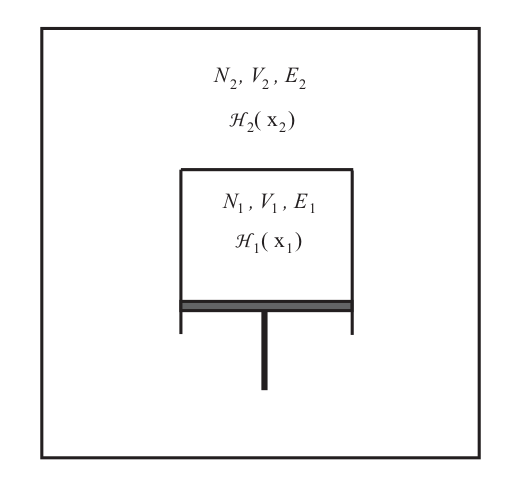
\includegraphics[scale=0.4]{isobar}
\label{fig:isobar}
\caption{Two systems in contact with a common thermal reservoir at temperature T. System
$1$ has $N_1$ particles in a volume $V_1$ ; system $2$ has $N_2$ particles in a volume $V_2$. Both $V_1$ and $V_2$ can vary.}
\end{figure}

\begin{multicols}{2}
	\begin{itemize}
		\item $E = E_1 + E_2\quad E_2\gg E_1$.
		\item $N = N_1 + N_2\quad N_2\gg N_1$.
		\item $V = V_1 + V_2\quad V_2\gg V_1$
		\item $\mathcal{H}(x) = \mathcal{H}_1(x_1) + \mathcal{H}_2(x_2)$.
	\end{itemize}
\end{multicols}


At fixed volumes $V_1$ and $V_2$:

$$Q(N, V, T) = C_N\int dx_1dx_2 e^{-\beta[\mathcal{H}_1(x_1) + \mathcal{H}_2(x_2)]} = g(N, N_1, N_2)C_{N_1}\int dx_1 e^{-\beta\mathcal{H}_1(x_1)}C_{N_2}\int dx_2 e^{-\beta\mathcal{H}_2(x_2)}$$

Which is the same expression for the micro canonical ensemble. $C_{N_1}$ and $C_{N_2}$ are the two constants that we would need to separate the system in two canonical ensemble with the same temperature $\beta$. 

The partition function for the system is: 

$$Q(N, V, T) \propto Q(N_1, V_1, T)Q(N_2, V_2, T)$$

But what happens if the volume is free to vary?

	\subsection{Phase space distribution}
	Combined system:

	$$f(x) = \frac{C_Ne^{-\beta\mathcal{H}(x)}}{Q(N, V, T)} = \frac{g(N, N_1, N_2)}{Q(N, V, T)}C_{N_1}e^{-\beta\mathcal{H}_1(x_1)}C_{N_2}e^{-\beta\mathcal{H}_2(x_2)}$$

We have to "wash out" the variables that describe the system $2$. So we need to integrate over the $x_2$ variables. 

	$$f(x_1) = \frac{g(N, N_1, N_2)}{Q(N, V, T)}C_{N_1}e^{-\beta\mathcal{H}_1(x_1)}C_{N_2}\int dx_2 e^{-\beta\mathcal{H}_2(x_2)} = \frac{Q_2(N_2, V-V_1, T)}{Q(N, V, T)}g(N, N_1, N_2)C_{N_1}e^{-\beta\mathcal{H}_1(x_1)}$$
	
	The quantity $C_{N_2}\int dx_2 e^{-\beta\mathcal{H}_2(x_2)}$ is exactly the partition function for the system $2$, considered as a canonical ensemble, with a fixed number of particles and a given volume and temperature. Thus being equal to $Q_2$: let's focus on this quantity. 

	First, the normalization is correct: $\int dV_1\int dx_1f(x_1, V_1) = 1$.
	
	Generally, we know that the partition function ($Q_2$ in this case) is equal to $e^{\beta[A]}$. So let's write this equation with the correct argument for the Helmholtz free energy. 

	$$\frac{Q_2(N_2, V-V_1, T)}{Q(N, V, T)} = e^{-\beta[A(N-N_1, V-V_1, T) - A(N, V, T)]}$$

Through a Taylor expansion:

	$$A(N-N_1, V-V_1, T) = A(N, V, T)-N_1\frac{\partial A}{\partial N}|_{N_1 = 0, V_1 = 0} = A(N, V, T)-\mu N_1 + PV_1$$
	
	The phase-space distribution for variable $x_1$ is:

	$$f(x_1) = g(N, N_1, N-N_1) e^{\beta\mu N_1}e^{-\beta P V_1}C_{N_1}e^{-\beta\mathcal{H}_1(x_1)}\qquad I_{N_1} = \frac{1}{V_0N_1!h^{3N_1}}$$

	We define a quantity $\Delta(N, P, T)$ to be the integral of hte entire phase-space, including the volume, of the constant $I_N$. The phase-space distribution is simply $e^{-\beta(\mathcal{H}(x) + PV)}$, so basically the analogous distribution function of the canonical ensemble, but instead of having the energy in the Boltzmann factor we have the enthalpy. 
	
	$$\Delta(N, P, T) = I_N\int_0^{\infty}dV\int dxe^{-\beta(\mathcal{H}(x) + PV)}\Rightarrow e^{\beta\mu N}\Delta(N, P, T) = 1$$
	
	Because of Euler (next chapter), the quantity $\mu N$ is exactly $G$:

	$$\Delta(N, P, T) = e^{-\beta\mu N} = e^{-\beta G(N, P, T)}$$
	
	Now we have an analogous relation: $e^{\beta A} \rightarrow e^{\beta G}$. 
	
	$$\Delta(N, P, T) = \frac{1}{V_0N!h^{3N}}\int_0^{\infty}dVe^{-\beta PV}\int dxe^{-\beta\mathcal{H}(x)} = \frac{1}{V_0}\int_0^{\infty}dVe^{-\beta PV}Q(N, V, T)$$
	
	\subsubsection{Further proof}
	A further proof that this is indeed a "good" system is provided, starting this time from the Gibbs free energy.

	$$G = A + P\langle V \rangle = \langle E + PV\rangle - TS = \langle\mathcal{H}(x) + PV\rangle + T\frac{\partial G}{\partial T}$$

We can obtain the average $langle E + PV\rangle$ by performing the average over the phase-space distribution we just introduced. We need to integrate over the volume and all the coordinates. The quantity $(\mathcal{H}(x) + PV)$ (remember that $V$ now is a constant) must be weighted by the corresponding Boltzmann factor, which includes not only the hamiltonian but also $PV$.

	$$\langle E + PV\rangle = \frac{I_N\int_0^{\infty} dV\int dx(\mathcal{H}(x) + PV)e^{-\beta(\mathcal{H}(x)+PV)}}{I_N\int_0^{\infty}dV\int dxe^{-\beta(\mathcal{H}(x) + PV)}} = -\frac{1}{\Delta(N, P, T)}\frac{\partial \Delta(N, P, T)}{d\beta} = -\frac{\partial\ln\Delta(N, P, T)}{\partial \beta}$$
	

	$$G(N, P, \beta) = -\frac{\partial\ln\Delta(N, P, \beta)}{\partial\beta}-\beta\frac{\partial G}{\partial \beta}$$

	If we plug in the following solution: $G(N, P, \beta) = -\frac{1}{\beta}\ln\Delta(N, P, \beta)$ in the previous differential equation we get $0$.
	
	We now have all the means to describe the system. 

	$$\langle V\rangle = \biggl(\frac{\partial G}{\partial P}\biggr)_{N, T}\qquad S = -\biggl(\frac{\partial G}{\partial T}\biggr)_{N, P}$$

	\subsection{Maxwell's square}
	
	Let's put everything into perspective. 

	We have seen in the NPT enseble that we can obtain the average volume as the derivative wrt pressure of the Gibbs free energy, the entropy can be taken as the derivative wrt temperature (keeping fixed N and T).
	\begin{multicols}{2}
		\begin{itemize}
			\item $\langle V\rangle = \biggl(\frac{\partial G}{\partial P}\biggr)_{N, T}$.
			\item $S = -\biggl(\frac{\partial G}{\partial T}\biggr)_{N, P}$.
		\end{itemize}
	\end{multicols}
	
	We also found the following equation from the isobaric-isoenthalpic ensemble:

	\begin{multicols}{2}
		\begin{itemize}
			\item $T = \biggl(\frac{\partial H}{\partial S}\biggr)_{N, P}$.
			\item $\langle V\rangle = \biggl(\frac{\partial H}{\partial P}\biggr)_{N, S}$.
		\end{itemize}
	\end{multicols}

The following are coming from the microcanonical ensemble :
	\begin{multicols}{2}
		\begin{itemize}
			\item $T = =\biggl(\frac{\partial U}{\partial S}\biggr)_{N, V}$.
			\item $P = - \biggl(\frac{\partial U}{\partial V}\biggr)_{N, S}$.
		\end{itemize}
	\end{multicols}
	
And the canonical ensemble:
	\begin{multicols}{2}
		\begin{itemize}
			\item $P = -\biggl(\frac{\partial A}{\partial V}\biggr)_{N, T}$.
			\item $S = - \biggl(\frac{\partial A}{\partial T}\biggr)_{N, V}$.
		\end{itemize}
	\end{multicols}

	\begin{figure}[H]
		
\includegraphics[scale = 0.1]{maxwell_square}
		\centering
		\caption{Maxwell's square}
	\end{figure}

 
	\subsection{Pressure viral theorem}
	The internal pressure that was calculated by the estimator was a function of all the coordinates and all the momenta. The internal pressure $P^{int}$ would be the average of this estimator. We want this quantity to be equal to the external pressure for the equations to be valid. 
	$$P^{(int)} =\langle\mathcal{P}(\vec{r}, \vec{p})\rangle = \biggl\langle\frac{1}{3V}\sum\limits_i\biggl[\frac{\vec{p}_i^2}{m_i} + \vec{F}_i\cdot\vec{r}_i\biggr]\biggr\rangle = kT\frac{\partial\ln Q}{\partial V}$$

To take average of this quantity for our new ensemble (NPT) we need to write down the partition function at the denominator and integrate over the volume. 

	\begin{align*}
		\langle P^{(int)}\rangle &= \frac{1}{\Delta(N, P, T)}\int_0^{\infty}dVe^{-\beta PV}Q(N, V, T)\frac{kT}{Q}\frac{\partial Q}{\partial V} = \frac{kT}{\Delta(N, P, T)}\int_0^{\infty}dVe^{-\beta PV}\frac{\partial Q}{\partial V}=\\
														 &= \frac{kT}{\Delta(N, P, T)}e^{-\beta PV}Q(N, V, T)|_0^{\infty}-\frac{kT}{\Delta(N, P, T})\int_0^{\infty}dV\biggl(-\frac{P}{kT}\biggr)e^{-\beta PV}Q(N, V, T) = \\
														 &=\frac{P}{\Delta(N, P, T)}\int_0^{\infty}dVe^{-\beta PV}Q(N, V, T) = P
	\end{align*}
	
	Consider the integration by parts of the quantity $\frac{kT}{\Delta(N, P, T)}e^{-\beta PV}Q(N, V, T)|_0^{\infty}$: when the volume tends to infinity the exponential goes to zero; when instead the volume is zero the partition function is zero, because there are no states where $V=0$. 
	We are left with only the second term and its integral is exactly $\Delta$. 
	Again, the quantity $dVe^{-\beta PV}Q(N, V, T)$ is equal to $\Delta$ and we get the external pressure $P$.
	We demonstrated that if we take the average of the internal pressure over the NPT ensemble we obtain exactly the external pressure $P$, which is expected.
	 This also means that if we want to compare what we get in the simulation with the external pressure that we are fixing, we should calculate the internal pressure and then calculate the average over many simulations.
	 
	 \paragraph{Take home message for the virial theorem: the volume-average internal pressure is equal to the external pressure}

	\subsection{Work virial theorem}
If we multiply the internal pressure for the volume (that changes):
	$$P^{(int)}V = kTV\frac{\partial \ln Q}{\partial V}$$
	
Then we obtain the same equations as before, but we need to include also the V:
	\begin{align*}
		\langle P^{(int)}V\rangle &= \frac{1}{\Delta(N, P, T)}\int_0^{\infty}dVe^{-\beta PV}Q(N, V, T)\frac{kTV}{Q}\frac{\partial Q}{\partial V} = \frac{kT}{\Delta(N, P, T)}\int_0^{\infty}dVe^{-\beta PV}V\frac{\partial Q}{\partial V} = \\
															&=\frac{kT}{\Delta(N, P, T)}e^{-\beta PV}VQ(N, V, T)|_{0}^{\infty}-\frac{kT}{\Delta(N, P, T)}\int_0^{\infty}dV\frac{\partial}{\partial V}(Ve^{-\beta PV})Q(N, V, T)=\\
															&= \frac{1}{\Delta(N, P, T)}\biggl[-kT\int_0^{\infty}dVe^{-\beta PV}Q(N, V, T) + P\int_0^{\infty}dV \, Ve^{-\beta PV}Q(N, V, T)\biggr]=\\
															&=-kT+P\langle V\rangle \Rightarrow \langle P^{(int)}V\rangle + kT = P\langle V\rangle
	\end{align*}
	
	The term $\int_0^{\infty}dV \, Ve^{-\beta PV}Q(N, V, T)$ is the average of the volume: the volume is multiplied by a weighting factor and divided by the partition function in the NPT ensemble. 
	The work is equal to the average quantity $\langle P^{(int)}V\rangle$, plus $kT$.
	Now, $kT$ indicates that is equaiton is the analogous of the equipartition theorem, but there's an extra degree of freedom, the varying volume. This is the reason why an additional $kT is present$.
	To be fair, $kT$ is very small and it does not change much the final equation.
	

	 \paragraph{Take home message for the work virial theorem: There is an extra degree of freedom, that is the volume.}
	
	These theorems are particularly important, since the algorithms we will see later are all written for the isobaric-isoenthlapic ensemble, but we can go to easily by adding a thermostat. 
	

\section{Andersen's Hamiltonian}
The best way to deal with the extra degree of freedom that (the volume) is to add it to the hamiltonian, as an extra variable, obviously with its own momentum.

This is the case of the Andersen's hamiltonian, defined as:

$$\mathcal{H}_A = \sum\limits_{i=1}^N\frac{V^{-\frac{2}{3}}\pi_i^2}{2m_i}+ U(V^\frac{1}{3}\vec{s}_1, \dots, V^{\frac{1}{3}}\vec{s}_N) + \frac{p_V^2}{2W} + PV\qquad W = (3N+1)kT\tau_b^2$$


We need to write down now Hamilton's equations, to obtain the time evolution for each of these coordinates:

\begin{itemize}
	\item $\dot{\vec{s}}_i = \frac{\partial \mathcal{H}_A}{\partial\pi_i} = \frac{V^{-\frac{2}{3}}\pi_i}{m_i}$.
	\item $\dot{\pi}_i = -\frac{\partial\mathcal{H}_A}{\partial\vec{s}_i} = -\frac{\partial U}{\partial (V^{\frac{1}{3}}\vec{s}_i)}V^{\frac{1}{3}}$.
	\item $\dot{V} = \frac{\partial\mathcal{H}_A}{\partial p_V}-\frac{p_V}{W}$.
	\item $\dot{p}_V = -\frac{\partial\mathcal{H}_A}{\partial V} = \frac{1}{3}V^{-\frac{5}{3}}\sum\limits_{i=1}^N\frac{\pi_i^2}{m_i}-\frac{1}{3}V^{-\frac{2}{3}}\sum\limits_{i=1}^N\frac{\partial U}{\partial(V^{\frac{1}{3}}\vec{s}_i)}\cdot\vec{s}_i-P$.
\end{itemize}

The derivative of $\dot{p}_V$ is slightly more complicated, since the dependence on $p$ is present on three terms. 

Inverting the transformation (the same inversion we performed to go from original coordinates to the scaled coordinates):

$$s_i = V^{-\frac{1}{3}}\vec{r}_i\Rightarrow \dot{\vec{s}}_i = V^{-\frac{1}{3}}\dot{\vec{r}}_i-\frac{1}{3}V^{-\frac{4}{3}}\dot{V}\vec{r}_i$$


$$\pi_i = V^{\frac{1}{3}}\vec{p}_i \Rightarrow \dot{\pi}_i = V^{\frac{1}{3}}\dot{\vec{p}}_i + \frac{1}{3}V^{-\frac{2}{3}}\dot{V}\vec{p}_i$$


We need to substitute these equation to the ones we previously derived:

\begin{itemize}
	\item $\dot{\vec{s}}_i = \frac{\partial \mathcal{H}_A}{\partial\pi_i} = \frac{V^{-\frac{2}{3}}\pi_i}{m_i} \rightarrow \dot{r}_i = \frac{p_i}{m_i} + \frac{\dot{V}}{3V} r_i$
	\item $\dot{\pi}_i = -\frac{\partial\mathcal{H}_A}{\partial\vec{s}_i} = -\frac{\partial U}{\partial (V^{\frac{1}{3}}\vec{s}_i)}V^{\frac{1}{3}} \rightarrow \dot{p}_i = - \frac{\partial U}{\partial r_i} - \frac{\dot{V} }{3V} p_i$ .
	\item $\dot{V} = \frac{\partial\mathcal{H}_A}{\partial p_V}-\frac{p_V}{W} \rightarrow \dot{V} = \frac{p_V}{W}$.
	\item $\dot{p}_V = -\frac{\partial\mathcal{H}_A}{\partial V} = \frac{1}{3}V^{-\frac{5}{3}}\sum\limits_{i=1}^N\frac{\pi_i^2}{m_i}-\frac{1}{3}V^{-\frac{2}{3}}\sum\limits_{i=1}^N\frac{\partial U}{\partial(V^{\frac{1}{3}}\vec{s}_i)}\cdot\vec{s}_i-P \rightarrow \dot{p}_V = \frac{1}{3V} \sum^N_{i=1} [\frac{p^2_i}{m_i} - \frac{\partial U}{\partial r_i} r_i] -P$.
\end{itemize}

Notice how the new term $ \frac{\dot{V}}{3V}$ accounts for the compressibility of the variable, letting it \textit{inflating} and \textit{deflating}.

Also notice that the last quantity is exactly the internal pressure estimator. We have now a variation in the momentum, that is conjugate to the volume, whenever the internal pressure differs from the external one ($\dot{p} != 0$).

The compressibility is equal to $0$ (incompressible).
To calculate the compressibility we need to take the derivative of $\dot{r}$ wrt $r_i$, yielding a factor which is $\frac{\dot{V}}{3V}$ for each particle and every degree of freedom (three for each particle). 

	\subsection{Andersen's equations}

	\begin{multicols}{2}
		\begin{itemize}
			\item $\dot{\vec{r}}_i = \frac{\vec{p}}{m_i} + \frac{\dot{V}}{3V}\vec{r}_i\Rightarrow\dot{\vec{r}}_i = \frac{\vec{p}_i}{m_i} + \frac{\dot{V}}{3V}\vec{r}_i$
			\item $\dot{\vec{p}}_i = -\frac{\partial U}{\partial\vec{r}_i} -\frac{\dot{V}}{3V}\vec{p}_i\Rightarrow \dot{\vec{p}}_i = -\frac{\partial U}{\partial\vec{r}_i}-\frac{\dot{V}}{3V}\vec{p}_i$.
			\item $\dot{V} = \frac{p_V}{W}\Rightarrow\dot{V} = \frac{p_V}{W}$.
			\item $\dot{p}_V = \frac{1}{3V}\sum\limits_{i=1}^N\biggl[\frac{\vec{p}_i^2}{m_i}-\frac{\partial U}{\partial\vec{r}_i}\cdot\vec{r}_i\biggr]-P\Rightarrow\dot{p}_V = \frac{1}{3V}\sum\limits_{i=1}^N\biggl[\frac{\vec{p}_i^2}{m_i}-\frac{\partial U}{\partial\vec{r}_i}\cdot\vec{r}_i\biggr]-P$.
		\end{itemize}
	\end{multicols}

	The conserved quantity:

	$$\mathcal{H}' = \sum\limits_{i=1}^N\frac{\vec{p}_i^2}{2m_i} + U(\vec{r}_1, \dots, \vec{r}_N) + \frac{p_V^2}{2W}+PV$$
	Notice how $\mathcal{H}'$ looks very similar to the enthalpy, aside from the kinetic energy part. 
	As usual, when we work in a system that is not hamiltonian (we started from a different hamiltonian, $\mathcal{H}'$ does not give back Anderson's equations) we need to derive the partition function:

	$$\Omega_P = \int dp_V\int_0^{\infty}\int d^N\vec{p}\int_{\mathcal{D}(V)}d^N\vec{r}\delta\biggl(\\mathcal{H}(\vec{r},\vec{p}) + \frac{p_V^2}{2W}+PV-H\biggr)$$

	Virial theorem:

	$$\biggl\langle\frac{p_V^2}{2W}\biggr\rangle = k\frac{T}{2}\Rightarrow \mathcal{H}(\vec{r},\vec{p}) + PV\text{ is conserved}$$
	
	The pressure (the average) will be kept constant, as for the enthalpy.

\section{MTK algorithm (NPT)}
One of the best choices for thermostatting the system is the MTK algorithm, developed by Martyna-Tobias-Klein in 1994. 
This algorithm introduces a new variable $\epsilon$:

$$\epsilon = \frac{1}{3}\ln\frac{V}{V_0}\Rightarrow\dot{\epsilon} = \frac{\dot{V}}{3V}=\frac{p_\epsilon}{W}$$

\begin{multicols}{2}
	\begin{itemize}
		\item $\dot{\vec{r}}_i = \frac{\vec{p}_i}{m_i} + \frac{p_\epsilon}{W}\vec{r}_i$.
		\item $\dot{\vec{p}}_i = -\frac{\partial U}{\partial\vec{r}_i} - \frac{p_\epsilon}{W}\vec{p}_i$.
		\item $\dot{V} = \frac{dVp_\epsilon}{W}$.
		\item $\dot{p}_\epsilon = dV(\mathcal{P}^{(int)}-P)$.
	\end{itemize}
\end{multicols}


Compressibility:

\begin{align*}
	\kappa & = \sum\limits_{i=1}^N\biggl[\frac{\partial}{\partial\vec{r}_i}\cdot\dot{\vec{r}}_i + \frac{\partial}{\partial\vec{p}_i}\cdot\dot{\vec{p}}_i\biggr] + \frac{\partial\dot{V}}{\partial V} + \frac{\partial\dot{p}_V}{\partial p_V} = \\
				 &= dN\frac{p_\epsilon}{W}-dN\frac{p_\epsilon}{W} = d\frac{p_\epsilon}{E} = \frac{\dot{V}}{V}
\end{align*}

To obtain incompressible equations that conserve $\mathcal{H}(\vec{r},\vec{p}) + PV + \frac{p_V^2}{2W}$ we need to apply some modifications:

$$\dot{\vec{p}}_i = -\frac{\partial U}{\partial\vec{r}_i} - \biggl(1+\frac{d}{N_F}\biggr)\frac{p_\epsilon}{W}\vec{p}_i\qquad \dot{p}_\epsilon = dV(\mathcal{P}^{(int)}-P) + \frac{d}{N_f}\sum\limits_{i=1}^N\frac{\vec{p}_i^2}{m_i}$$

With $F$ being the number of degrees of freedom of the system. 

	\subsection{Langevin piston}
	In many programs and applications, we will use the Langevin thermostat. 
	The only difference from the Andersen's equations is the last one, with a friction acting on the volume and a last term representing a random force (or "kick"). 

	\begin{itemize}
		\item $\dot{\vec{r}}_i = \frac{\vec{p}_i}{m_i} + \frac{\dot{V}}{3V}\vec{r}_i$.
		\item $\dot{\vec{p}}_i = -\frac{\partial U}{\partial\vec{r}_i}-\frac{\dot{V}}{3V}\vec{p}_i$.
		\item $\dot{V} = \frac{p_V}{W}$.
		\item $\dot{p}_V = \frac{1}{3V}\sum\limits_{i=1}^N\biggl[\frac{\vec{p}_i^2}{m_i}-\frac{\partial U}{\partial\vec{r}_i}\cdot\vec{r}_i\biggr]-P-\gamma\dot{V}+R(t)$.
	\end{itemize}

	$$\langle R(0)R(t)\rangle = \frac{2\gamma kT}{W}\delta(t)$$
	
	The Langevin piston is mostly preferred as a barostat (it will not be thoroughly described though, as its equations are more complicated).
	
\section{Summary}
\begin{itemize}
\item We constructed the formalism of the isobaric ensembles, starting by performing the Legendre transform of the micro canonical ensemble to obtain the isobaric-isoenthalpic esnable; then the same reasoning was applied to the canonical ensemble to obtain the isobaric - isothermal (NPT) ensemble.
\item We demonstrated that the steps and the reasoning to modify the equations of the micorcanonical ensemble to go to the canonical ensemble, apply pretty much in the same way also for isobaric-isoenthalpic for the NPT. 
\item In the NPT ensemble we can calculate everything like a canonical ensemble, however the volume is now a variable. 
\item the pressure virial theorem, important for molecular simulations, and work virial theorem, useful for the derivation of Andersen's hamiltonian, were introduced. 
\end{itemize}
